\documentclass[12pt]{paper}
\usepackage{mathptmx} % Nearly Times New Roman
\usepackage[acronym,toc]{glossaries}
\include{acros}
%\makeglossaries
%%%%%%%%%%%%%%%%%%%%%%%%%%%%%%%%%%%

\usepackage{color}
\usepackage{subcaption}
\usepackage{graphicx}
\usepackage{booktabs} % nice rules for tables
\usepackage{microtype} % if using PDF
\usepackage{xspace}
\usepackage{listings}
\usepackage{textcomp}
\usepackage{multicol,tabularx,capt-of}
\usepackage{multirow}
%\usepackage{ulem}
\usepackage{pdflscape}
% Page length commands go here in the preamble
\setlength{\oddsidemargin}{-0.25in} % Left margin of 1 in + 0 in = 1 in
\setlength{\textwidth}{7in}   % Right margin of 8.5 in - 1 in - 6.5 in = 1 in
\setlength{\topmargin}{-.75in}  % Top margin of 2 in -0.75 in = 1 in
\setlength{\textheight}{9.2in}  % Lower margin of 11 in - 9 in - 1 in = 1 in



\definecolor{listinggray}{gray}{0.9}
\definecolor{lbcolor}{rgb}{0.9,0.9,0.9}
\definecolor{burgundy}{rgb}{0.5, 0.0, 0.13}
\definecolor{burntorange}{rgb}{0.8, 0.33, 0.0}
\definecolor{chromeyellow}{rgb}{1.0, 0.65, 0.0}
\definecolor{darkred}{rgb}{0.55, 0.0, 0.0}

\lstset{
    %backgroundcolor=\color{lbcolor},
    language={C++},
    tabsize=4,
    rulecolor=\color{black},
    upquote=true,
    aboveskip={1.5\baselineskip},
    belowskip={1.5\baselineskip},
    columns=fixed,
    extendedchars=true,
    breaklines=true,
    prebreak=\raisebox{0ex}[0ex][0ex]{\ensuremath{\hookleftarrow}},
    frame=single,
    showtabs=false,
    showspaces=false,
    showstringspaces=false,
    basicstyle=\scriptsize\ttfamily\color{green!40!black},
    keywordstyle=\color[rgb]{0,0,1.0},
    commentstyle=\color[rgb]{0.133,0.545,0.133},
    stringstyle=\color[rgb]{0.627,0.126,0.941},
    numberstyle=\color[rgb]{0,1,0},
    identifierstyle=\color{black},
    captionpos=t,
}

\newcommand{\code}[1]{\lstinline[basicstyle=\ttfamily\color{green!40!black}]|#1|}
\newcommand{\units}[1] {\:\text{#1}}%
\newcommand{\SN}{S$_N$}
\newcommand{\cyclus}{\textsc{Cyclus}\xspace}
\newcommand{\Cyclus}{\cyclus}
\newcommand{\citeme}{\textcolor{red}{CITE}\xspace}
\newcommand{\TODO}[1] {{\color{red}\textbf{TODO: #1}}}%

\newcommand{\comment}[1]{{\color{green}\textbf{#1}}}

%%%%%%%%%%%%%%%%%%%%%%%%%%%%%%%%%%%
\begin{document}


%\begin{frontmatter}
\title{Evaluating computational methods for modeling off-normal operation of gas centrifuge cascades}

% Authors. Separated by commas
\author{
  Baptiste Mouginot,
  Kathryn Mummah,
  Paul P.H. Wilson}


\date{}
% Institutes of the authors
\institution{$^1$Department of Nuclear Engineering and Engineering Physics,
University of Wisconsin-Madison}
%\\$^2$Sandia National Laboratories}
\maketitle


% 0.Abstract

\begin{abstract}
\begin{itshape}
    This work compares and evaluates different computational approaches for modeling
off-normal operation of a gas centrifuge enrichment cascade.

The goal of this work focuses on developing the necessary understanding of
potential misuse of enrichment cascades, contributing to more effective
international safeguards designs and approaches.  While it is straightforward to
design a symmetric enrichment cascade under ideal conditions as a function of the
theoretical feed, product and tails assays, it is very difficult to find
reliable information about the behavior of a given cascade when the feed assay
does not match the design value. Several methods have been developed to assess
the behavior of an enrichment cascade in such circumstances. In addition to the
cut ($\theta$) those methods evaluate the feed to product, feed to tails and the
product to tails enrichment ratio, respectively, $\alpha$, $\beta$ and $\gamma$,
as a function of the cascade feed assay. As those four parameters depend on each
other, determining two of them fully defines the other.  The first approach
consists of fixing $\theta$ and $\alpha$ recomputing the corresponding assays at
each stages of the cascade. The second one maintains the ideal condition of the
cascade ($\alpha$ and $\beta$ fixed across the whole cascade), modifying
$\theta$ value at each stage accordingly. Both approaches have been implemented
into the Cyclus fuel cycle simulator\cite{cyclus, mbmore.2018}. The third fixes
$\theta$ and $\gamma$, using both $\alpha$ and $\beta$ at each stage as free
parameters. The third method has been investigated in \cite{walker.2017}.

Following a description of each method and an evaluation of differences between
each approach, this work compares the results produced by these methods within
scenarios involving misuse of symmetric enrichment cascades simulated using the dynamic
nuclear fuel cycle simulator, Cyclus.
\end{itshape}

\end{abstract}


% I.   Motivation
\section{Motivation}

Gas centrifuge cascades are usually designed to operate in an ideal manner, with
no losses in separative work. To achieve such ideal configuration, the cascade
is designed to be fed with a specific feed assay and produce the target
enrichment while rejecting tails at a fixed assay.

With the current international tensions regarding enrichment capabilities, this
work aims to measure the effectiveness of an enrichment cascade when used outside of
its designed scope and quantify the attractiveness of such way to build up
significant quantity of \gls{HEU}.

The present work investigates the performance of an enrichment cycle when chaining
gas enrichment cascades tuned for low enrich uranium production from natural
uranium. As literature on the mater is for obvious reason limited, three
behavior models have been implemented and used to evaluate the response of an
enrich cascade when fed with different assays than the design one. This work
also takes advantage of the Cyclus\cite{cyclus} fuel cycle capabilities to
evaluate the assay values at equilibrium.



% II.  Theory
%   a. cascade design
%   b. miss-use model
%       i.   case A
%       ii.  case B
%       iii. case C
\section{Theory}
\subsection{Centrifuge properties}

The present work uses the analytical solution by R\"aetz \cite{raetz.phd} of the
differential equation for the gas centrifuge as described in \cite{glaser.2008}.
Centrifuge parameters, such as average gas temperature, $T$, peripheral speed,
$v$, height, $h$, diameter, $d$, pressure ratio, $x$, feed flow rate, $F$,
counter-current flow ratio, $L/P$, and efficiency, $e$ have been chosen (Table
\ref{tab:centrifuges}) to match the cascade design describe in
\cite{glaser.2008} and \cite{walker.2017} using P1-type centrifuges.

\begin{table}[htb]
\centering
\caption{Summary of the centrifuge parameters.}
\begin{tabular}{cccccccc}
\toprule
$T$[K] & $v$[m/s]    & $h$[m] & $d$[m]   & $x$   & $F$[mg/s]  & $L/F$ & $e$  \\
\midrule
320    & $320$       & $1.8$  & $0.105$  & $10^{3}$ & $13$       & 2     & 1.0  \\
\bottomrule
\end{tabular}

  \label{tab:centrifuges}
\end{table}

\subsection{Cascade Design}

The cascade is built as an ideal cascade, with no losses in the separative work,
which corresponds to $\alpha =\beta = const$ for all stages of the cascade, where
$\alpha$ and $\beta$ respectively represent the feed to product and the feed to
tails enrichment factors.  $\alpha$ and $\beta$ can be expressed as function of
the abundance ($R$) or the enrichment ($N$) of respectively the product
($R'$, $N'$) and the feed ($R$, $N$) and the feed and the tails ($R''$, $N''$) such
as:
\begin{subequations} \label{eq:alphabeta}
    \begin{equation} \label{eq:alpha_def}
        \alpha = \frac{R'}{R} = \frac{N'}{1-N'}\frac{1-N}{N} 
\end{equation}
\\
\begin{equation}\label{eq:beta-def}
        \beta = \frac{R}{R''} = \frac{N}{1-N}\frac{1-N''}{N''} 
\end{equation}
\end{subequations}

As detailed in \cite{avery} it is also possible to derive $\alpha$ from the
first principle, and express it as a function of the feed rate $F$, the
separative performance $\delta U(\theta)$ and the cut $\theta$:

    \begin{equation} \label{eq:alpha}
    \alpha = \sqrt{\frac{2\delta U}{F} \frac{1-\theta}{\theta}}+1
\end{equation}

From the mass conservation, $N = \theta N' + (1-\theta)N''$, and equations
\eqref{eq:alphabeta} it is possible to express $\beta$ as a function of the
feed abundance, $R$, the cut $\theta$ and $\alpha$:

\begin{equation}\label{eq:beta}
    \beta =   R \left(\dfrac{1-\theta}
                     {\dfrac{R}{R+1}- \theta \dfrac{\alpha R}{1+\alpha R}} -1\right)
\end{equation}


From equation \eqref{eq:alpha} and \eqref{eq:beta} it is possible to determine
the cut, $\theta$ required to build an ideal cascade:
\begin{eqnarray}
    \theta_{i} = \dfrac{N_{i} - \dfrac{1}{1 + \beta/R_{i}}}{ \dfrac{\alpha R_{i}}{1 + \alpha R_{i}} -
           \dfrac{1}{1 + \beta/R_{i}}}
           \label{eq:theta}
\end{eqnarray}

As $\alpha_{i}$ and $\beta_{i}$ remain constant, only the value of the cut,
$\theta_{i}$, changes across the different stages of a cascade.  This algorithm
assumes that the corresponding separative power $\delta U$ (not re-computed) can
be achieved with the chosen centrifuge design, tuning other operational
parameter such as the rotation speed, the counter-current flow ratio, etc.  Once
$\theta_{i}$ is determined, it is possible to compute the product and the tail
assay.

The design of the cascade is performed through 2 steps.  First one determines
the configuration and number of stages, adding stages until the product assay of
the final stage is greater or equal the product targeted assay, and similarly
the tails assay is less or equal the tails desired assay.  This determines the
number of enriching and stripping stages as well as their enrichment properties
($N_{i}$, $N'_{i}$, $N''_{i}$,$\theta_{i}$i).


The second step determines the relative flows at each stages, solving the linear
flow equation, \eqref{eq:flow}.
The cascade can then be populated with actual machines until the maximum number
available of machines is reached.

\begin{equation}
\setcounter{MaxMatrixCols}{20}
\begin{bmatrix}
     -1        & 1-\theta_{_{S+1}} & 0 & ...  & 0              & 0              & 0                 & 0                 & 0                 & ...  & 0               & 0 \\
 \theta_{_{S}} & -1                & 0 & ...  & 0              & 0              & 0                 & 0                 & 0                 & ...  & 0               & 0 \\
               &                   &   &     &                &                & ...               &                   &                   &     &                 &   \\
 0             & 0                 & 0 & ...  & \theta_{_{-2}} & -1             & 1 - \theta_{_{0}} & 0                 & 0                 & ...  & 0               & 0 \\
 0             & 0                 & 0 & ...  & 0              & \theta_{_{-1}} & -1                & 1 - \theta_{_{1}} & 0                 & ...  & 0               & 0 \\
 0             & 0                 & 0 & ...  & 0              & 0              & \theta_{_{0}}     & -1                & 1 - \theta_{_{2}} & 0   & ...             & 0 \\
               &                   &   &     &                &                & ...               &                   &                   &     &                 &   \\
 0             & 0                 & 0 & ...  & 0              & 0              & 0                 & 0                 & 0                 & ...  & -1              & 1-\theta_{_{E}} \\
 0             & 0                 & 0 & ...  & 0              & 0              & 0                 & 0                 & 0                 & ...  & \theta_{_{E-1}} & -1
 \end{bmatrix}
 \times
 \begin{bmatrix}
     F_{_{S}}   \\
     F_{_{S+1}} \\
     \cdots     \\
     F_{_{-1}}  \\
     F_{_{0} }  \\
     F_{_{1} }  \\
     \cdots     \\
     F_{_{E-1}} \\
     F_{_{E}}
 \end{bmatrix}
 =
 \begin{bmatrix}
     0      \\
     0      \\
     \cdots \\
     0      \\
     F      \\
     0      \\
     \cdots \\
     0      \\
     0
\end{bmatrix}
%\caption{caption needed!}
\label{eq:flow}
\end{equation}



\subsection{Misuse models}

Little information is available about optimising an existing enrichment cascade
that is being fed with a feed enrichment that does not match the design one. So
far 3 different methods have been investigated. 

The first one assumes that no change are been made on the cascade, i.e $\delta
U$, $F$ and $\theta$ are fixed across all stages. The second one assumes the cut
value at each stage is retuned to maintain the ideal state of the cascade,
$\alpha$ and $\beta$ remain fixed. The last one, described in \cite{walker.2017}
assumes the tails to product enriching factor and the cut remain constants ($\gamma =
\alpha\times\beta$). Models behaviors and assumptions are summarized in Tab.
\ref{tab:models}.

\begin{table}[htb]
\centering
  \caption{Summary of misuse model properties.}
\begin{tabular}{l|ccc}
\toprule

Model                &    A                 & B                  & C  \\
\midrule
Constant parameters  & $\alpha_i, \theta_i$ & $\alpha_i=\beta_i$ & $\gamma_i=\alpha_i .\beta_i, \theta_i$       \\
Varying parameters   & $\beta_i$            & $\theta_i$         & $\alpha_i, \beta_i$                     \\
Assays determination & blended              & ideal              & blended                  \\
Flow                 & unchanged            & reduced            & unchanged       \\

\bottomrule
\end{tabular}
  \label{tab:models}
\end{table}


\subsubsection{Model A}

The tuning method A does not re-optimize $\theta_i$ keeping the same flow as the
ideal configuration. From equation \eqref{eq:alpha}, maintaining $\delta U$, $F$
and $\theta$ unchanged implies $\alpha$ remains unchanged as well. According to
equation \eqref{eq:beta}, when $\alpha$ and $\theta$ are fixed, if the feed
assay ($N$) changes, $\beta$ will change accordingly.  This breaks the
ideal status of the cascade, i.e. $N_{i} \neq N'_{i-1} \neq N''_{i+1}$.


In order to compute the proper product and tails assay at each stage, the tails
and the product from the next and the previous stage respectively must be
blended in order to determine the correct stage feed assay. All feed assays are
iteratively updated, blending the proper product and tails, then using the
updated feed assay, the new product and tails assays are recomputed. This
process is repeated until the sum of the square difference in assays is smaller
than $10^{-8}$.  As the cut remain fixed at each stage the flows do not need to
be recomputed.

This model assumes that it is possible to maintain the separative power of a
centrifuges, $\delta U$, for any feed assays $N$ while maintaining its cut
$\theta$ and feed flow $F$.

\subsubsection{Model B}

Using the second method, the cut value at each stage $\theta_i$, is retuned in
order to maintain the $\alpha_i$ and $\beta_i$ at their original values
(equation \eqref{eq:theta}). The cascade remaining ideal, the product and tails
assay at each stages are easily determined using equations \eqref{eq:alphabeta}.

As the cut values change, the relative flow rates between the different stage
are recomputed using equation \eqref{eq:flow}. The flow rates are determinted as
the largest flow rates allowed by the cascade design, number of centrifuges
limiting the flow at each stage.

This model assumes that it is possible to tune a centrifuge separative power
$\delta U$, for any feed assay $N$, cut $\theta$ and feed flow $F$, in order to
maintain its constant feed to product enrichment factor $\alpha$.




\subsubsection{Model C}
The last model assumes that the tails to product enrichment factor remains
constant regardless to the feed assays. To compute the response of the cascade
one need to determine $\alpha$ and $\beta$ such that their product and
$\theta$ remain fixed. 
From equations \eqref{eq:alphabeta} and the assay conservation equation $N =
\theta N' + (1-\theta)N''$ it is possible to express the product $N'$ as a function of
the feed assay $N$, $\gamma$ and the cut $\theta$ as one solution of the second
order equation \eqref{eq:gamma_p}:

\begin{equation}\label{eq:gamma_p}
    \theta(\gamma-1)N'^2+((N+\theta)(\gamma-1)+1)N'-N\gamma = 0
\end{equation}


The only solution allowing product assay to range between 0 and 1 is the
following :
\begin{equation}\label{eq:model_b_sol}
    N' = \frac{N+\theta}{2\theta} +
         \frac{1 - \sqrt{\gamma^{2}(N-\theta)^{2}
                         + 2\gamma( N^{2} + N - \theta^{2} + \theta)
                         + (N + \theta + 1)^{2}}}
              {2\theta(\gamma - 1)}
\end{equation}
Once the product assay is known, one can trivially determine the tails assay,
$\alpha$ and $\beta$ using equations \eqref{eq:alphabeta} and mass
conservation.

Similar to model A, because the cut values remain constant, the flows don't
need to be recomputed, and the correct assays, $\alpha$ and $\beta$ are
determined through iterative blending of the product assays of the previous
stage and the tails assay of the next stage using equation
\eqref{eq:model_b_sol}.

This model assumes that it is possible to tune the centrifuge separative power
$\delta U$ in order to maintain, for any feed assay $N$, its tails to product
enrichment factor $\gamma$, while maintaining its cut $\theta$ and feed flow
$F$.



% III. Experiement
%   a.  cycle 
%   b.  cascade per level optimisation
\section{The experiment}
This works focuses on comparing the different miss use models to a reference
calculation in which a single large cascade is build and designed to directly
produce \gls{HEU} from natural uranium.
This works uses the Cyclus fuel cycle simulator to allow material exchange
between facilities.

\subsection{The cascade configuration}
\subsubsection{reference}
As mentioned previously, all the further calculations will be compared to the
most favorable configuration to produce \gls{HEU}, where all the available
centrifuges are used in a single large cascade designed to directly produce \gls{HEU}
from natural uranium, with a tail assay close to $0.3w\%$ uranium. The design
characteristic of the reference cascade are summarized in Table
\ref{tab:cascade_config}.

\subsubsection{default cascade}
The default cascade is the cascade design for normal civilian enrichment
operation, enriching natural uranium to about $3.5w\%$. This cascade will be
layered and fed with uranium at higher enrichment to evaluate the possibility
to used them, with few or no tuning, to produce \gls{HEU}. The characteristics of
the default cascade are summarized in Table \ref{tab:cascade_config}.

\begin{table}[htb]
\centering
  \caption{Summary of cascade design.}
\begin{tabular}{cccc}
\toprule

Cascade Design &       & Reference  & Default    \\
\midrule
Targeted  & Feed       & $0.71w\%$  & $0.71w\%$  \\
Assays    & Product    & $90w\%$    & $4.0w\%$   \\
          & Tail       & $0.3w\%$   & $0.3w\%$   \\
\midrule
Effective & Product    & $90.35w\%$ & $4.13w\%$  \\
Assays    & Tail       & $0.28w\%$  & $0.28w\%$  \\ 
\midrule
Stages    & Enriching  & 4          & 4          \\
Number    & Stripping  & 39         & 10         \\
\bottomrule
\end{tabular}
  \label{tab:cascade_config}
\end{table}


\subsection{scenarios}
Seven different simulations have been simulated:
\begin{itemize}
\item one as the reference calculation, with a single centrifuges designed to
    produce directly \gls{HEU} from natural uranium,
\item three calculations (one per miss-use model) were default cascade are
    chained to produce \gls{HEU}, without recycling the tails of each cascade,
    the cascade tails are directly sent to the waste,
\item three calculations (one per miss-use model) were default cascade are
    chained to produce \gls{HEU}, the tails of each cascade are recycled, blending
    the tail of one level in the feed of the previous level of
    cascades (see Figure \ref{fig:cascade_level}.
\end{itemize}
In the following, cascades can be connected in tandem, where each set of cascade
in parallel is called a ``level``, as illustrated on Figure
\ref{fig:cascade_level}.

\begin{figure}[ht] % replace 't' with 'b' to force it to be on the bottom
    \centering
    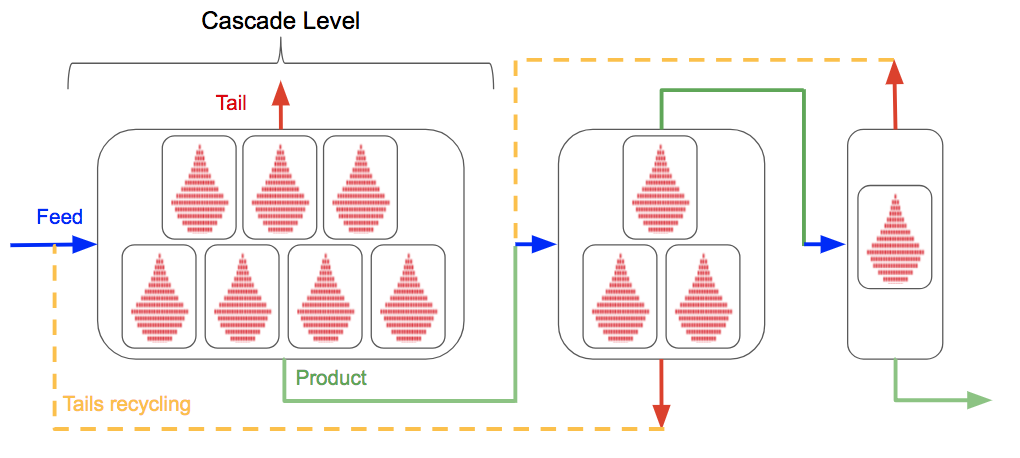
\includegraphics[scale=0.45]{flow}
    \caption{Schematic representation of the chained cascades with three levels,
    with the feed, product and the tail flows, respectively in blue, green and
    red. The dashed orange line represent the alternative tail flow with
    recycling them.}
    \label{fig:cascade_level}
\end{figure}


\subsection{Level population}
In order to assign the optimum number of cascade to each level a virtual cut as
been computed as:
\begin{equation}
    \theta^{v}_{i} = \frac{F_{i}-T_{i}}{P_{i}-T_{i}},
\end{equation}
where, i represents a level of cascade and $F_{i}$, $P_{i}$ and $T_{i}$
respectively the feed, product and tail assay of the cascades at this level.

A flow equation similar to \eqref{eq:flow} is then solve to get the optimum
number of cascade per level. When the tail are not recycled, the $(1-\theta)$
terms are removed from the flow equation.  The results of the level population
are summarized in Table \ref{tab:level}.

\subsection{Timestep effect}

As it can be observed on Figures \ref{fig:case1}, \ref{fig:case2} and
\ref{fig:case3}, the different cascade levels required up to $2n+1$, with $n$ the
level number to start enriching uranium. This corresponds to the time required
for the material to propagate from the natural uranium source to the level,
regardless of the duration of the timestep (hour, day, month,...). This is also
true for the number of timestep required to reach the equilibrium assays value in
the tail reprocessing cases. This is why one will only consider equilibrium
values.


% IV.  results
%   a. time step effects
%   b. no tail recycling
%   c. tail recycling
\section{Results}

\subsection{Miss-use modeling}

\begin{table}[h!]
\centering
  \caption{Summary of cascades level population.}
\begin{tabular}{ccccccccc}
\toprule

Model       &        &           & A/NR      & A/R       & B/NR      & B/R      & C/NR       & C/R          \\
%Recycling   &        &           & No        & yes       & No        & Yes     & No        & yes        \\
\midrule                                                                                                 
        &            & Feed      & $0.71w\%$ & $1.3w\%$  & $0.71w\%$ & $0.94w\%$ & $0.71w\%$ & $1.33w\%$ \\
Level 0 & Assay      & Product   & $4.13w\%$ & $7.7w\%$  & $4.13w\%$ & $5.43w\%$ & $4.13w\%$ & $4.82w\%$ \\
        &            & Tails     & $0.29w\%$ & $0.5w\%$  & $0.29w\%$ & $0.39w\%$ & $0.29w\%$ & $0.55w\%$ \\
        & Cascades   &           & 25        & 25        & 25        & 24        & 25        & 25        \\
\midrule                                                                                                 
        &            & Feed      & $4.13w\%$ & $11.9w\%$ & $4.13w\%$ & $6.84w\%$ & $4.13w\%$ & $12.2w\%$ \\
Level 1 & Assay      & Product   & $22.8w\%$ & $55.7w\%$ & $20.6w\%$ & $30.7w\%$ & $22.9w\%$ & $58.5w\%$ \\
        &            & Tails     & $1.8w\%$  & $6.6w\%$  & $1.72w\%$ & $2.91w\%$ & $1.81w\%$ & $6.52w\%$ \\
        & Cascades   &           & 3         & 4         & 3         & 4         & 3         & 4         \\
\midrule                                                                                                 
        &            & Feed      & $22.8w\%$ & $55.7w\%$ & $20.6w\%$ & $34.3w\%$ & $22.9w\%$ & $58.5w\%$ \\
Level 2 & Assay      & Product   & $78.5w\%$ & $95.0w\%$ & $61.0w\%$ & $75.8w\%$ & $82.0w\%$ & $97.0w\%$ \\
        &            & Tails     & $4.13w\%$ & $50.9w\%$ & $9.56w\%$ & $17.5w\%$ & $15.7w\%$ & $53.8w\%$ \\
        & Cascades   &           & 1         & 1         & 1         & 1         & 1         & 1         \\
\midrule                                                                                                 
        &            & Feed      & $78.5w\%$ & N.A.      & $61.0w\%$ & $75.8w\%$ & $82.3w\%$ & N.A.      \\
Level 3 & Assay      & Product   & $98.2w\%$ & N.A.      & $90.4w\%$ & $95.0w\%$ & $99.1w\%$ & N.A.      \\
        &            & Tails     & $76.1w\%$ & N.A.      & $79.3w\%$ & $56.1w\%$ & $80.3w\%$ & N.A.      \\
        & Cascades   &           & 1         & N.A.      & 1         & 1         & 1         & N.A.      \\
\bottomrule
\end{tabular}
  \label{tab:level}
\end{table}

As illustrated in Figures \ref{fig:assays} and summarized on Tab
\ref{tab:level}, the different model don't have the same effect on the cascade
behavior. While the models A and C, allow a quick enrichment gain, with the
cascades chaining, respectively 4/23/78/98 and 4/23/82/99, the model B, the
enrichment gain is only 4/21/61/90. 


\begin{figure}[h!]
    \centering
    \begin{subfigure}[t]{0.45\textwidth}
        \centering
        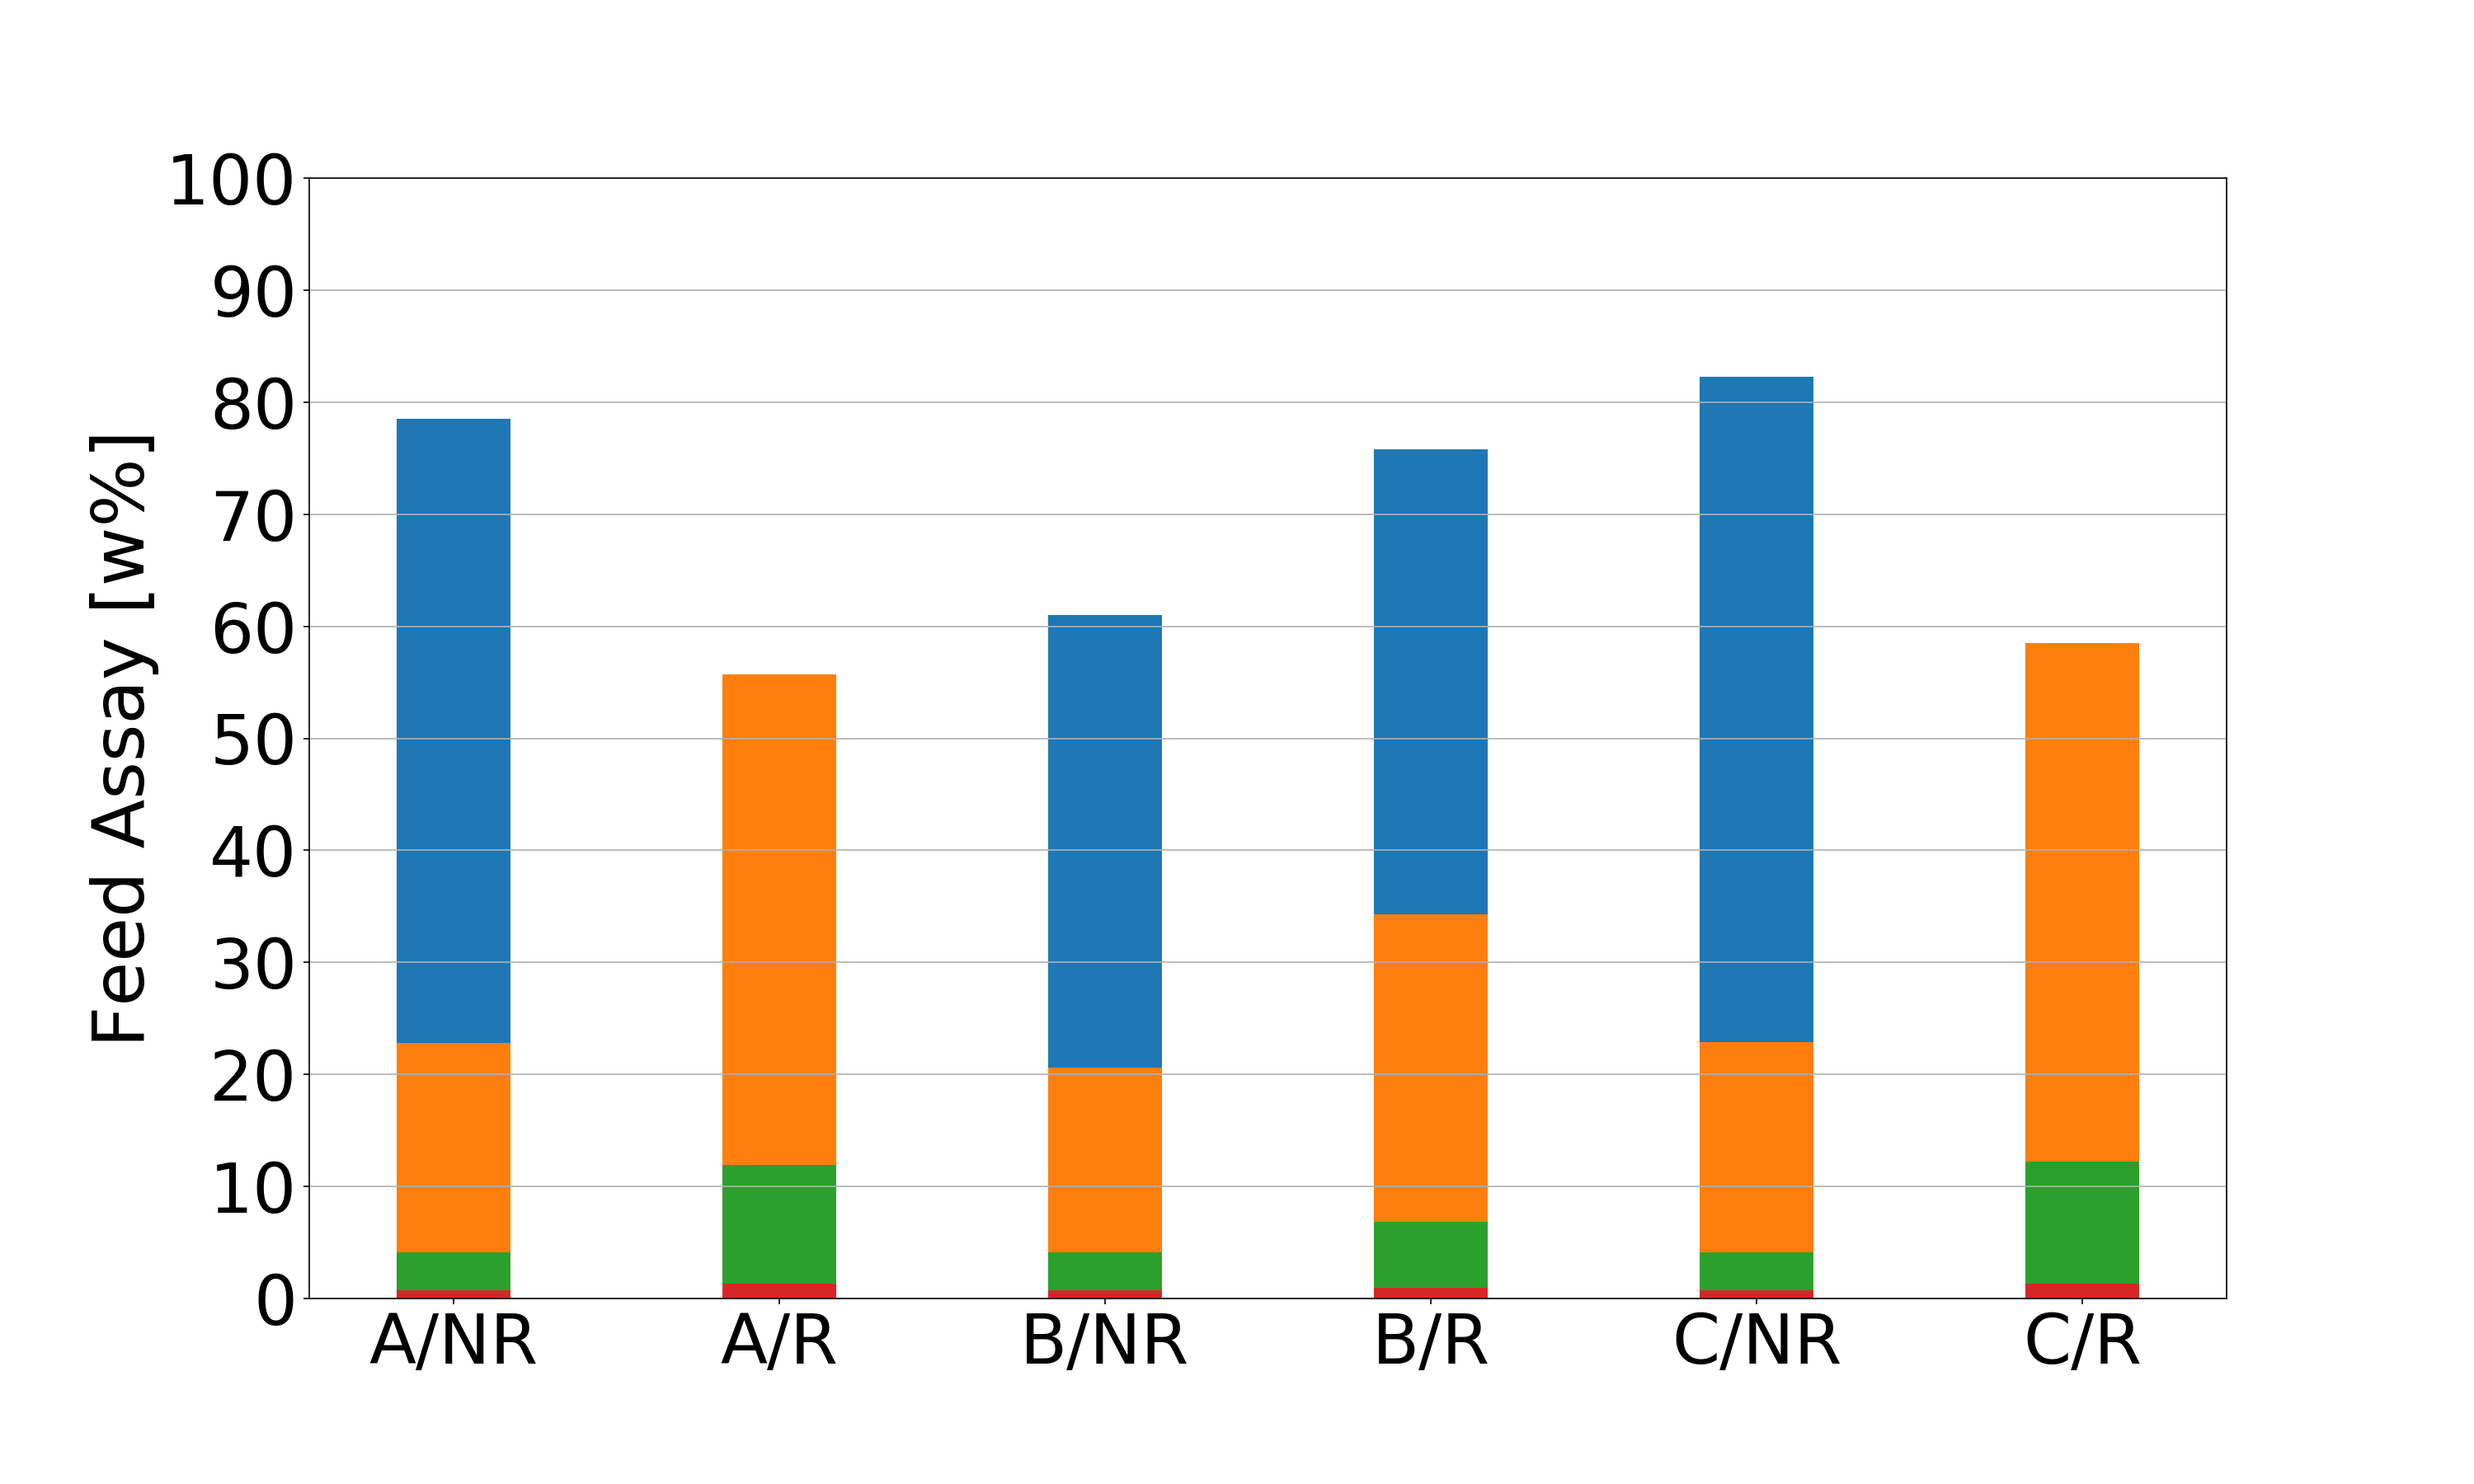
\includegraphics[scale=0.2]{feed_assays}
        \caption{Feed Assays.}
        \label{sfig:feed_assay}
    \end{subfigure}%
    \begin{subfigure}[t]{0.45\textwidth}
        \centering
        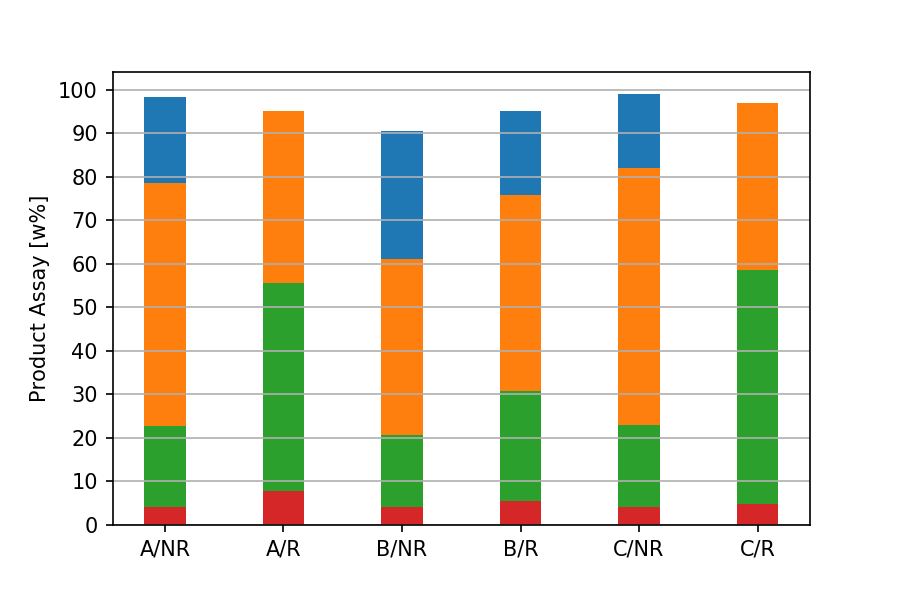
\includegraphics[scale=0.2]{product_assays}
        \caption{Product Assays.}
        \label{sfig:product_assay}
    \end{subfigure}
    \begin{subfigure}[t]{0.45\textwidth}
        \centering
        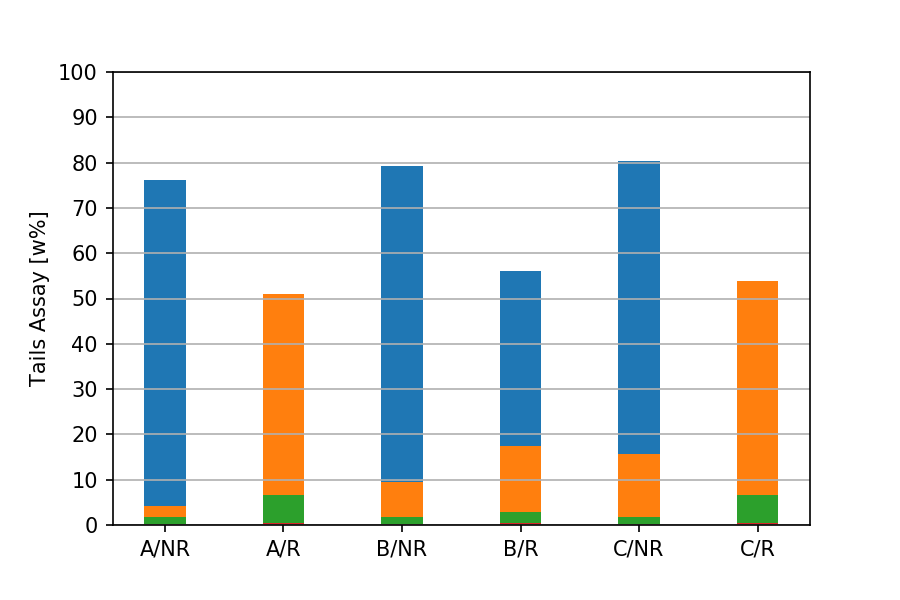
\includegraphics[scale=0.2]{tails_assays}
        \caption{Tails Assays.}
        \label{sfig:tails_assay}
    \end{subfigure}
    \caption{Feed (\subref{sfig:feed_assay}), product
        (\subref{sfig:product_assay}) and tails assays (\subref{sfig:tails_assay})
        in $m\%$ of $^{235}$U, per cascade level from 0 to 3 (red, green, orange,
        blue), per model (A/B/C) and without/with tails recycling (NR/R). The
        black dashed line represents the $90 m\%$ enrichment threshold.}
    \label{fig:assays}
\end{figure}



\subsection{Tails recycling}

As shown in Figures \ref{fig:assays}, recycling the tails increases the overall product assay at
all the different levels. As the tails assay of a level $n+1$ is always higher than
the product assay of the level $n-1$, recycling the tails of level $n+1$ will
consequently increase the feed assay of level $n$ (see Table \ref{tab:level}).
Moreover, with an increased feed assay, tails and product assays increase as
well, increasing de facto the feed assays of respectively cascade levels $n-1$
and $n+1$, etc.  This effect reduces the number of cascade levels required to reach
\gls{HEU} in case A and C.



\subsection{\gls{HEU} Production}

As shown in Figure \ref{fig:HEU_rate}, recycling increases the final \gls{HEU}
production rate, from $2$ to almost $20$ kg/y when using models A and C, and from
$17$ to $38$ kg/y with the model B. For the reference calculation where all the
available cascades are used within a single large cascade design for direct
\gls{HEU} production, the \gls{HEU} production rate is slightly over $50$ kg/y.


As models A and C, rely on maintaining the cut values at each stages of the
cascade and share the same number of levels, have the exact same cascade
repartition across the different levels and the same \gls{HEU} production rate.

\begin{figure}[h!] % replace 't' with 'b' to force it to be on the bottom
    \centering
    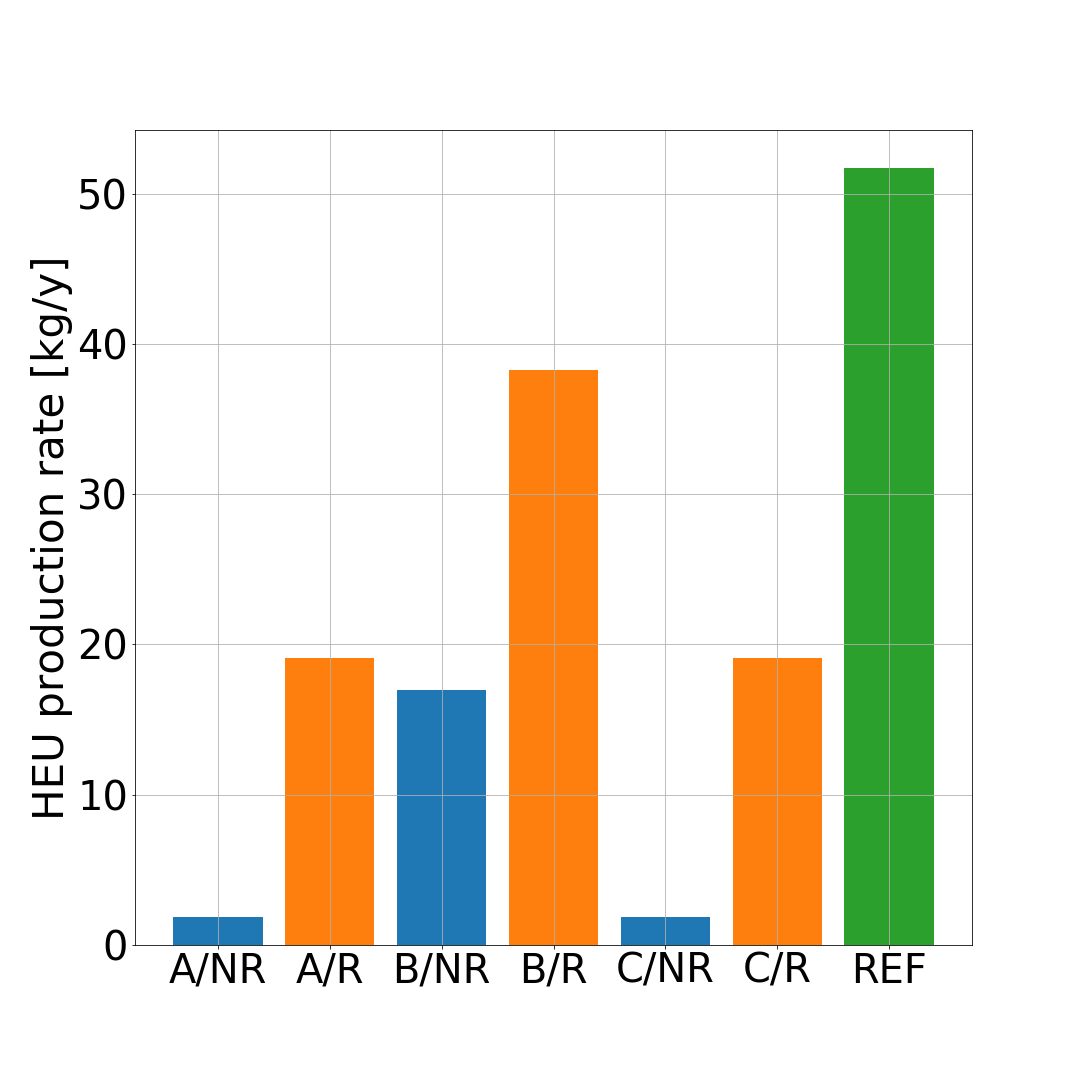
\includegraphics[scale=0.25]{HEU_prod_rate}
    \caption{Production rate at equilibrium for the different model
        configurations, the case without tails recycling (blue), with tails
        recycling (orange), and the reference one (green). A-B-C represent
        the model used, and NR-R the case without tails recycling and the case
        with tails recycling, respectively.}
    \label{fig:HEU_rate}
\end{figure}


% V.  Discussion
% VI. Conclusions and future plan
\section{Discussion}

It is really interesting to observe that when the cascade is left completely
untouched (Model A) or when it is slightly retuned to maintain the tail to
product enrichment factor as well as the cut of each centrifuges (Model C),
chaining the cascade we can observe high increase of the enrichment at each
level.  On the contrary, when retuning the cut of each centrifuges to maintain
the ideal state of the cascades (Model B) while chaining them, the \gls{HEU}
production rate is favored over the enrichment gain.

The tail recycling allows for each model a huge gain in productivity, even for
then model B where the number of levels required to reach $90w\%$ of $^{235}$U
in the uranium does not change. Even if no cascades chaining allows to retrieve
the same production rate as a direct enrichment, the model B with tail
reprocessing reach about $80\%$ of an optimum production, which is far from
being negligible, allowing to build up a Significant Quantity of \gls{HEU} in
less than 8 months\ldots


\section{Conclusion and future works}

This works has investigated and quantify the difference between potential
retuning of a gaseous enrichment cascade in order to chain them to produce
\gls{HEU} initially tuned to produce uranium enrichment for commercial reactors.
One of this tuning method allows up to $80\%$ of the production rate of a single
large enrichment cascade designed specifically for \gls{HEU} production using
the same number of centrifuges.

This works will be extended to the near future with additional miss-use method,
allowing for example the reconfiguration of the centrifuges in the cascades.

For this study, the usage of the Cyclus fuel cycle simulator was not really
required, it only allows a quick determination of the blending equilibrium. It
is planned to make use of the Cyclus Dynamical Resource Exchange full capability
in order to automatically assign the different cascades to the different level
as function of the resources availability, optimising the productions rates in
each cases.

While mathematically correct, the authors do not guaranty the feasibility
different miss-use tuning methods implemented and are welcoming any insight on
the matter.






%\end{frontmatter}


%\input{appendix}

%%%%%%%%%%%%%%%%%%%%%%%%%%%%%%%%%%%%%%%%%%%%%%%%%%%%%%%%%%%%%%%%%%%%%%%%%%%%%%%%
\begin{small}
\bibliographystyle{ans}
\bibliography{refs}  % NO SPACES BETWEEN BIB FILENAMES!
\end{small}
\end{document}
